\section{Design Concepts}

We learned from our investigation that it is slow for users to hit the right key on a virtual keyboard due to the lag in visual feedback and limited proprioception.   We thus propose Slide, described below, to speed up text entry by using relative positioning and reducing the need for accuracy through auto-correction. 

\begin{comment}

Our design efforts focused on balancing three of the above factors: input speed, learning time, and physical size.
Our thinking was particularly influenced by the interaction design of cell phones that use T9 input, which relies on a database of words to disambiguate cell phone keypad keystrokes that are associated with more than one letter.
If we could design an input device that combined the best of the standard keyboard (fast text input, familiar layout) and the 12-key cell phone keypad (small size), we would have a device that could be used in off-the-desktop situations, potentially for extended typing tasks, with little degradation in performance. 

Despite the difficulties for the users to physically locate their finger outside of the virtual environment in order to interact with the keyboard on a mobile phone, the users are not completely helpless from their previous typing experience.
To start with, the users have muscle memory from typing on traditional mobile keyboards. With this previous experience, the user remembers, although imprecise, the location of letters if the layout of the keyboard is the same as what they are used to.

Thus, to leverage these previous knowledge of the users and address the problem that the users cannot physically see their fingers, we center our designs around two key features that we believe can help them adjust to typing in virtual reality: relative finger tracking, and batched keys.

Traditional mobile keyboard requires users to tap on the key precisely to enter an individual letter.
This method falls prey to specifically to the problem described above: users cannot tap on the individual keys accurate enough because they cannot see their finger relative to the touch screen of the mobile phone in a virtual environment.
Thus, 
\end{comment}

\subsection{Relative Vectors as Key Entries}

To minimize the need for visual feedback, we propose to use relative positioning.  Relative movement, instead of absolute, has also been found to be beneficial in reducing fatigue~\cite{Hincapie-Ramos:2014:CEM:2556288.2557130} so the user can start the interaction from their current position. 

The virtual keyboard in Slide is laid out exactly as the original keyboard, so the users are already familiar with the placement of the keys.   The positioning of the keyboard is relative to the user's first touch.  No matter where the finger is placed on the touchpad, it is assumed to touch the center of the keyboard, right between the ``f'' and ``g'' letters.  To enter a letter, the user slides his finger to the key of interest.  As he lifts his finger, the key is entered.  Because of the familiarity of the keyboard layout, the user knows roughly even without looking at the keyboard.  Visual feedback is provided by showing the virtual keyboard and the trail his finger makes.   

Text entry in Slide is different from swiping in several important ways. 
\begin{enumerate}
\item
With swiping, the user enters a word through a continuous movement, connecting pairs of consecutive letters.  Without good visual feedback, the drift in our sense of our finger position accumulates with each letter.   With Slide, every letter input is independent.  The user needs only to slide always from the center of the keyboard to the letter of interest.  

\item 
As discussed above, we need to discard the first letter entry when we swipe in VR, since users cannot hit the first key correctly.   No such special provision is needed for Slide.

\item
With swiping, the worst-case distance traveled for each letter is the full length of the keyboard.  The worst case in Slide is just half the length of the keyboard. 
\end{enumerate}


\subsection{Directions as Key Entries}

\begin{figure}
  \centering

  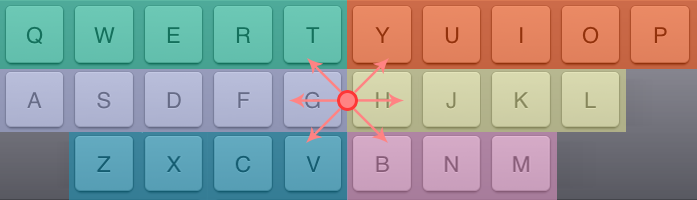
\includegraphics[width=1\columnwidth]{figures/arrows}
  
  \caption{The six tiles of the direction-based keyboard.}
  ~\label{fig:swipeVRLayout}
\end{figure}

While an improvement over swiping, the technique proposed above still requires the user to slide his finger precisely to the right key, which can be half the length of the keyboard.  We reduce the accuracy required of the user by relying on auto-correction.  We divide the keyboard into 6 tiles, as shown in Figure~\ref{fig:swipeVRLayout}.   The user only needs to slide his finger in the direction of the tile that contains the key of interest.  It is easy to indicate the direction accurately, with a minimum distance traveled for all keys, without visual feedback. 

We use a Bayesian word recommender to infer the most probable words among words that correspond to the same tile sequence.  For example, the words ``hello'' and ``jelly'' has the same representation.  
This recommender algorithm use 2-gram and 3-gram data from Google Books Ngram Viewer\footnote{http://storage.googleapis.com/books/ngrams/books/datasetsv2.html}, part of speech frequency for English dictionary, individual word frequency for the entire English language, and produces a prediction score.
The word with highest prediction score will be selected by default as the most probable word.  
The whole word is presented all at once, instead of a letter at a time, and the user is given the option to choose a less probable word among the possibilities, as shown in Figure~\ref{fig:multiword}.  


\begin{figure}
  \centering

  \includegraphics[width=.4\columnwidth]{figures/multiword}
  
  \caption{Users are presented with words represented by the same sequence of tile inputs.}
  ~\label{fig:multiword}
\end{figure}

\subsection{A Hybrid Keyboard}

While the directional approach is faster, it lacks the precision necessary for entering numbers, punctuations, or words not in the dictionary, such as user names, passwords, and URLs.   Our solution is to use the relative-vector technique as a backup for the direction-based keyboard.  Since both these techniques have the same keyboard layout, the user simply can mix these two entry techniques easily.  Our keyboard automatically detects the user's intention based on the speed with which the keys are entered. 

In addition, we introduce a few shortcuts for the frequently used ``delete'' and ``space'' keys.   Users can double tap the touch screen to indicate delete.  For the space key, the user can click a specific physical button on the controller, such as the ``trigger'' button on the bottom side of the Vive controller.  We have also experimented automatically inserting a space after a certain timeout period between 150 and 500 ms.  However, we found that users preferred to have the control of when to insert the space themselves.   

\begin{figure}
  \centering
  \begin{subfigure}{.6\columnwidth}
  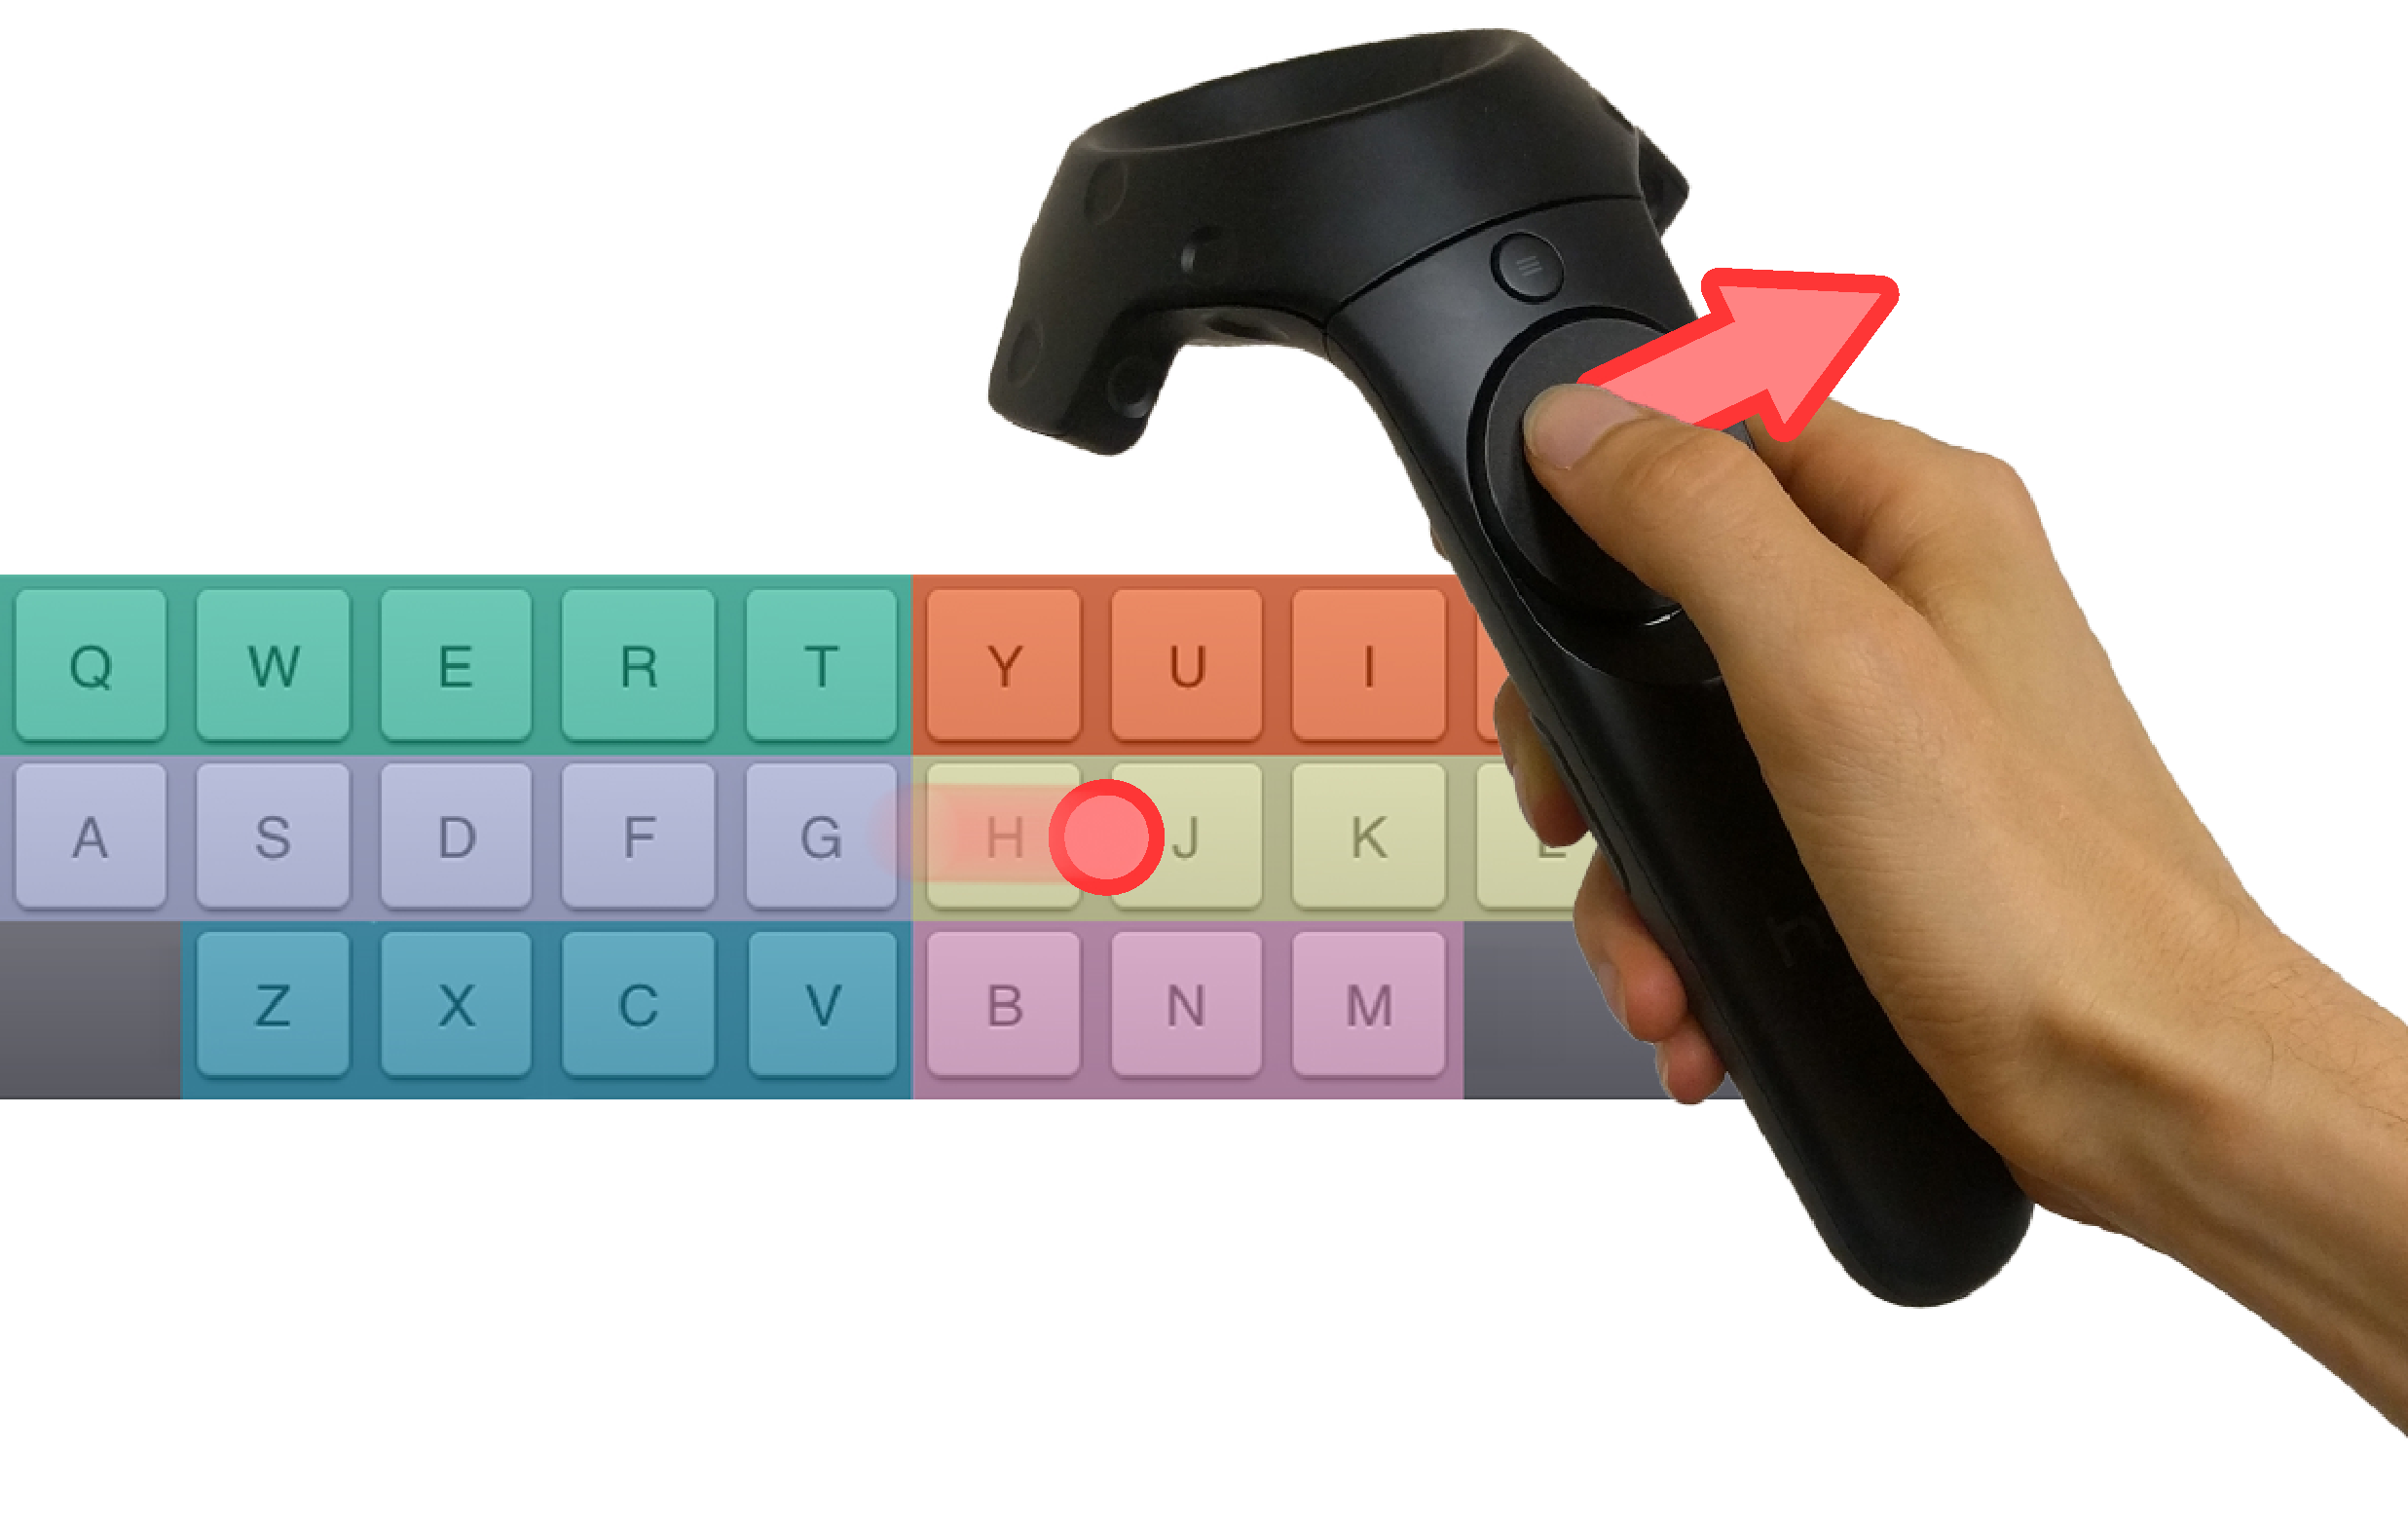
\includegraphics[width=\textwidth]{figures/right}
  \caption{Slide right to enter \textit{h}. }
  \label{fig:controllerVive}
  \end{subfigure}
  \\
  \begin{subfigure}{.6\columnwidth}
  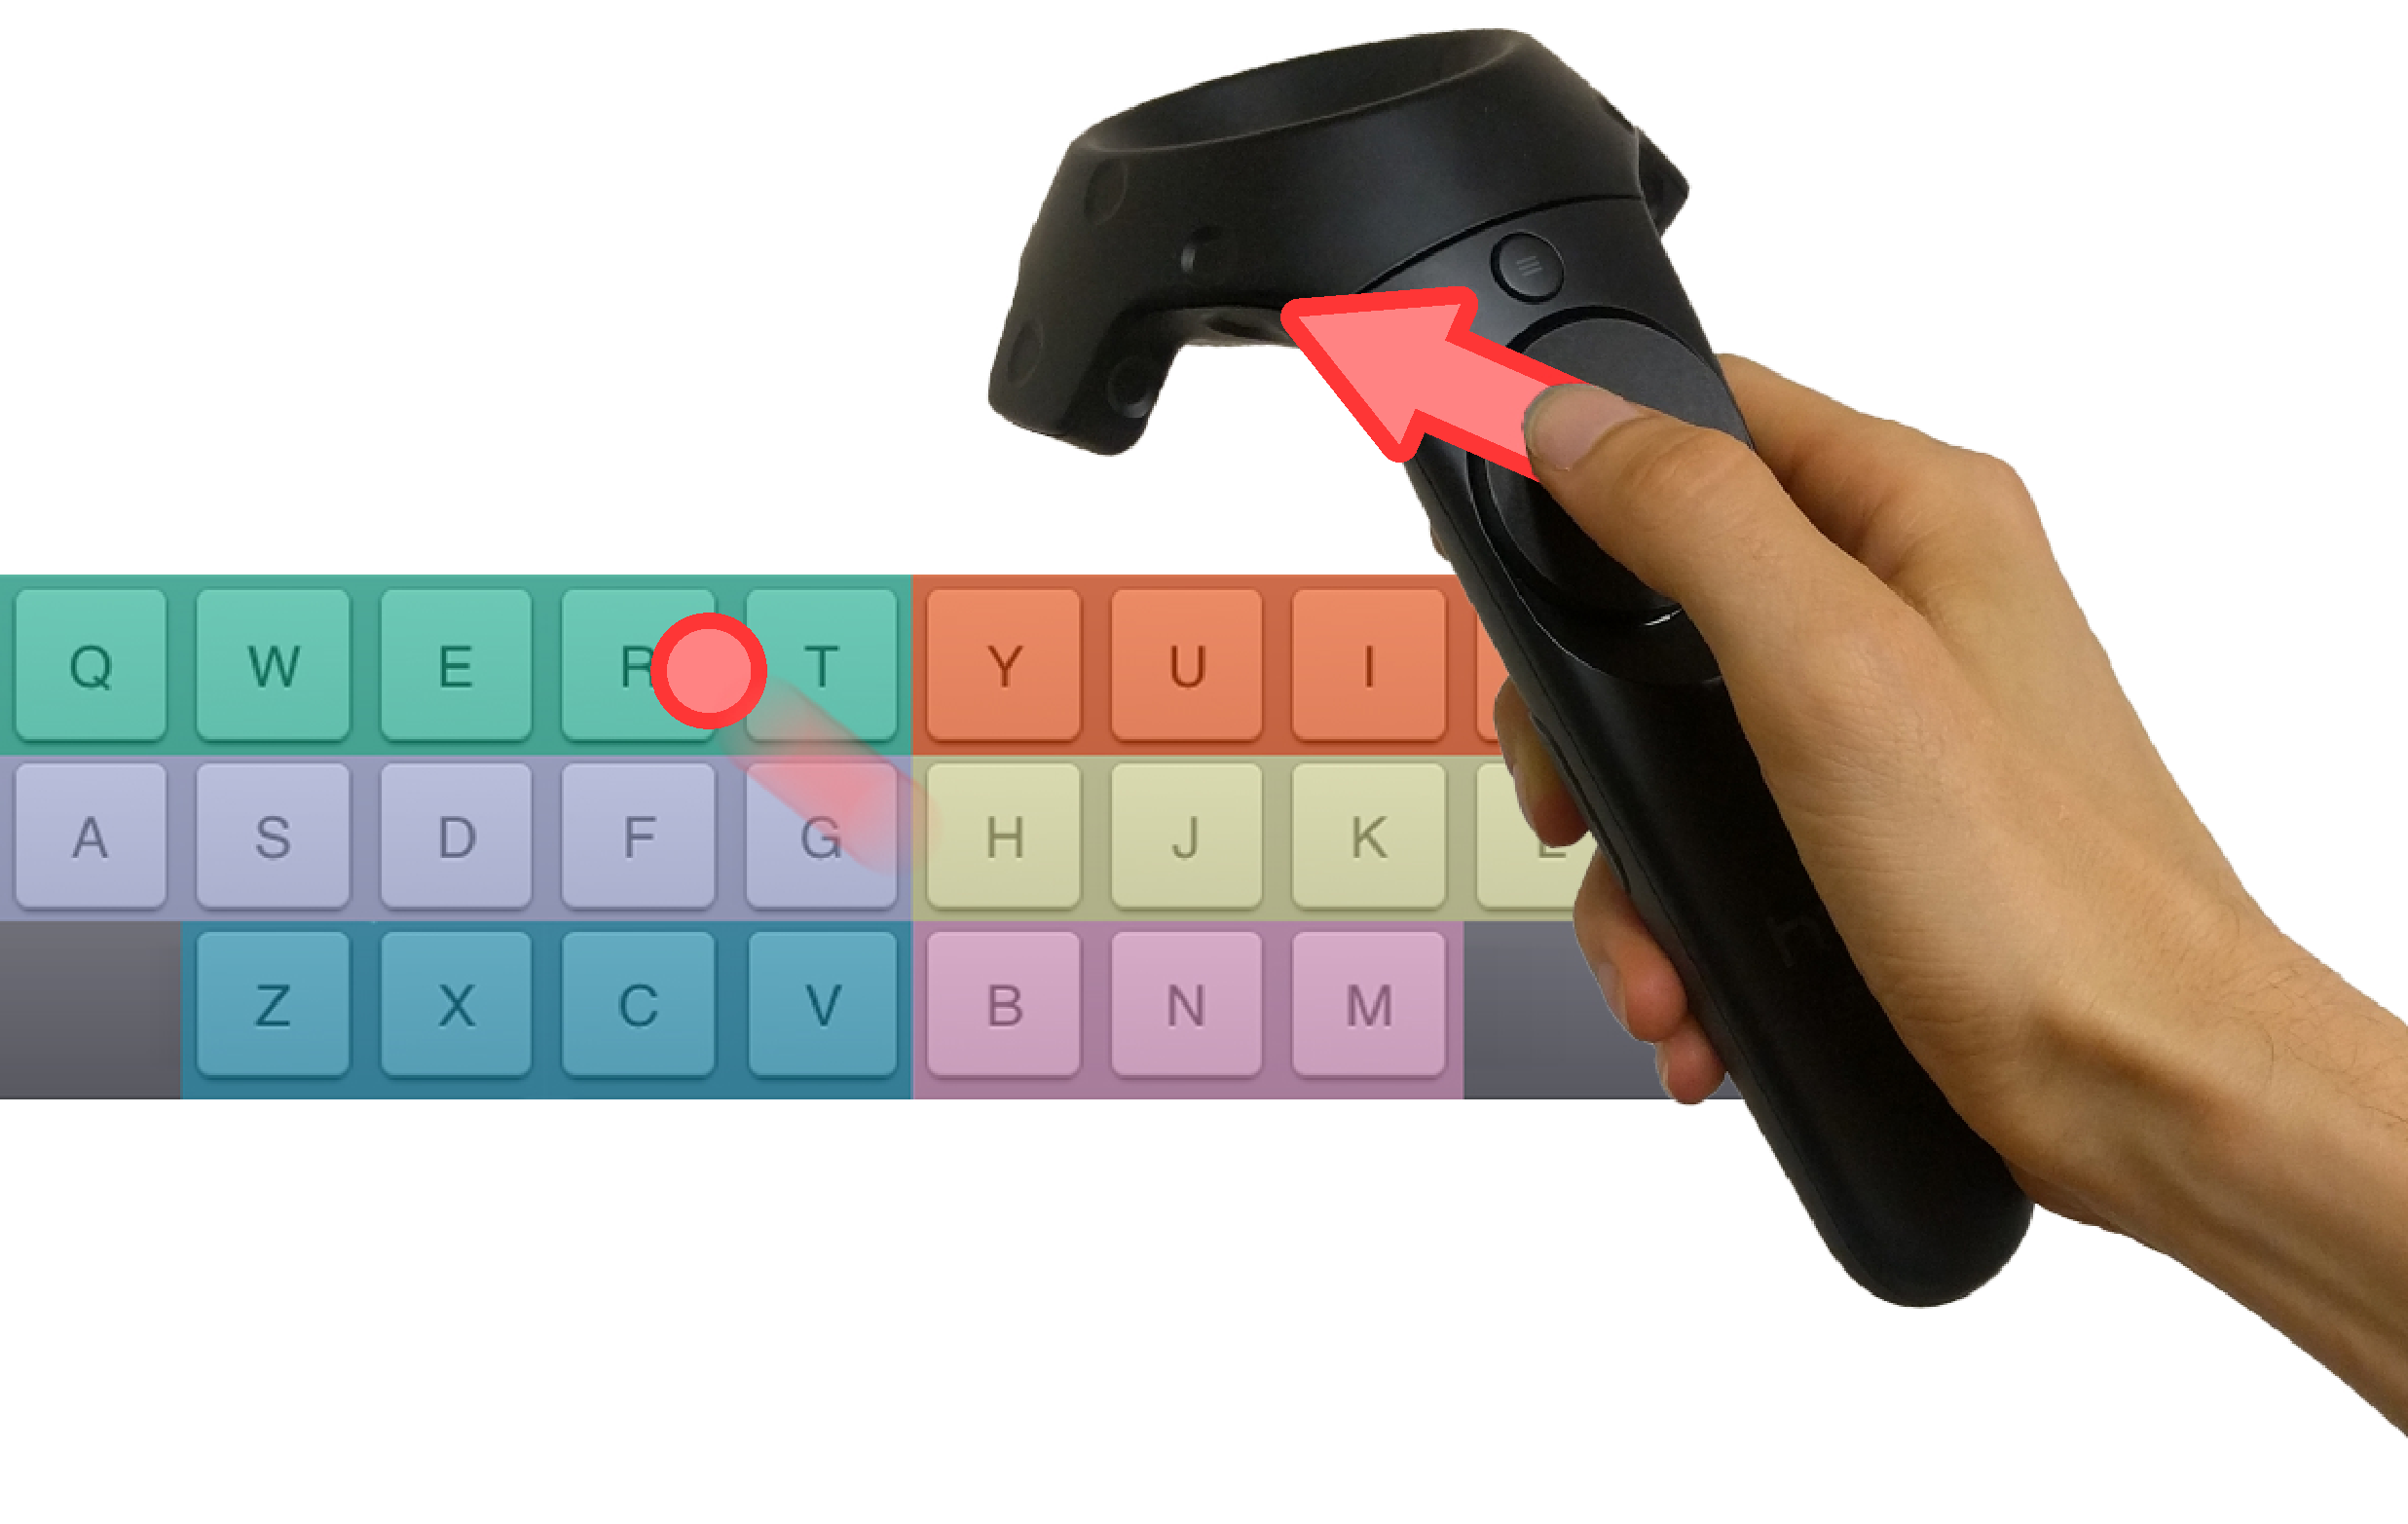
\includegraphics[width=\textwidth]{figures/upperLeft}
  \caption{Slide right to enter \textit{e}. }
  \label{fig:controllerVive}
  \end{subfigure}
  \\
  

  \begin{subfigure}{.6\columnwidth}
  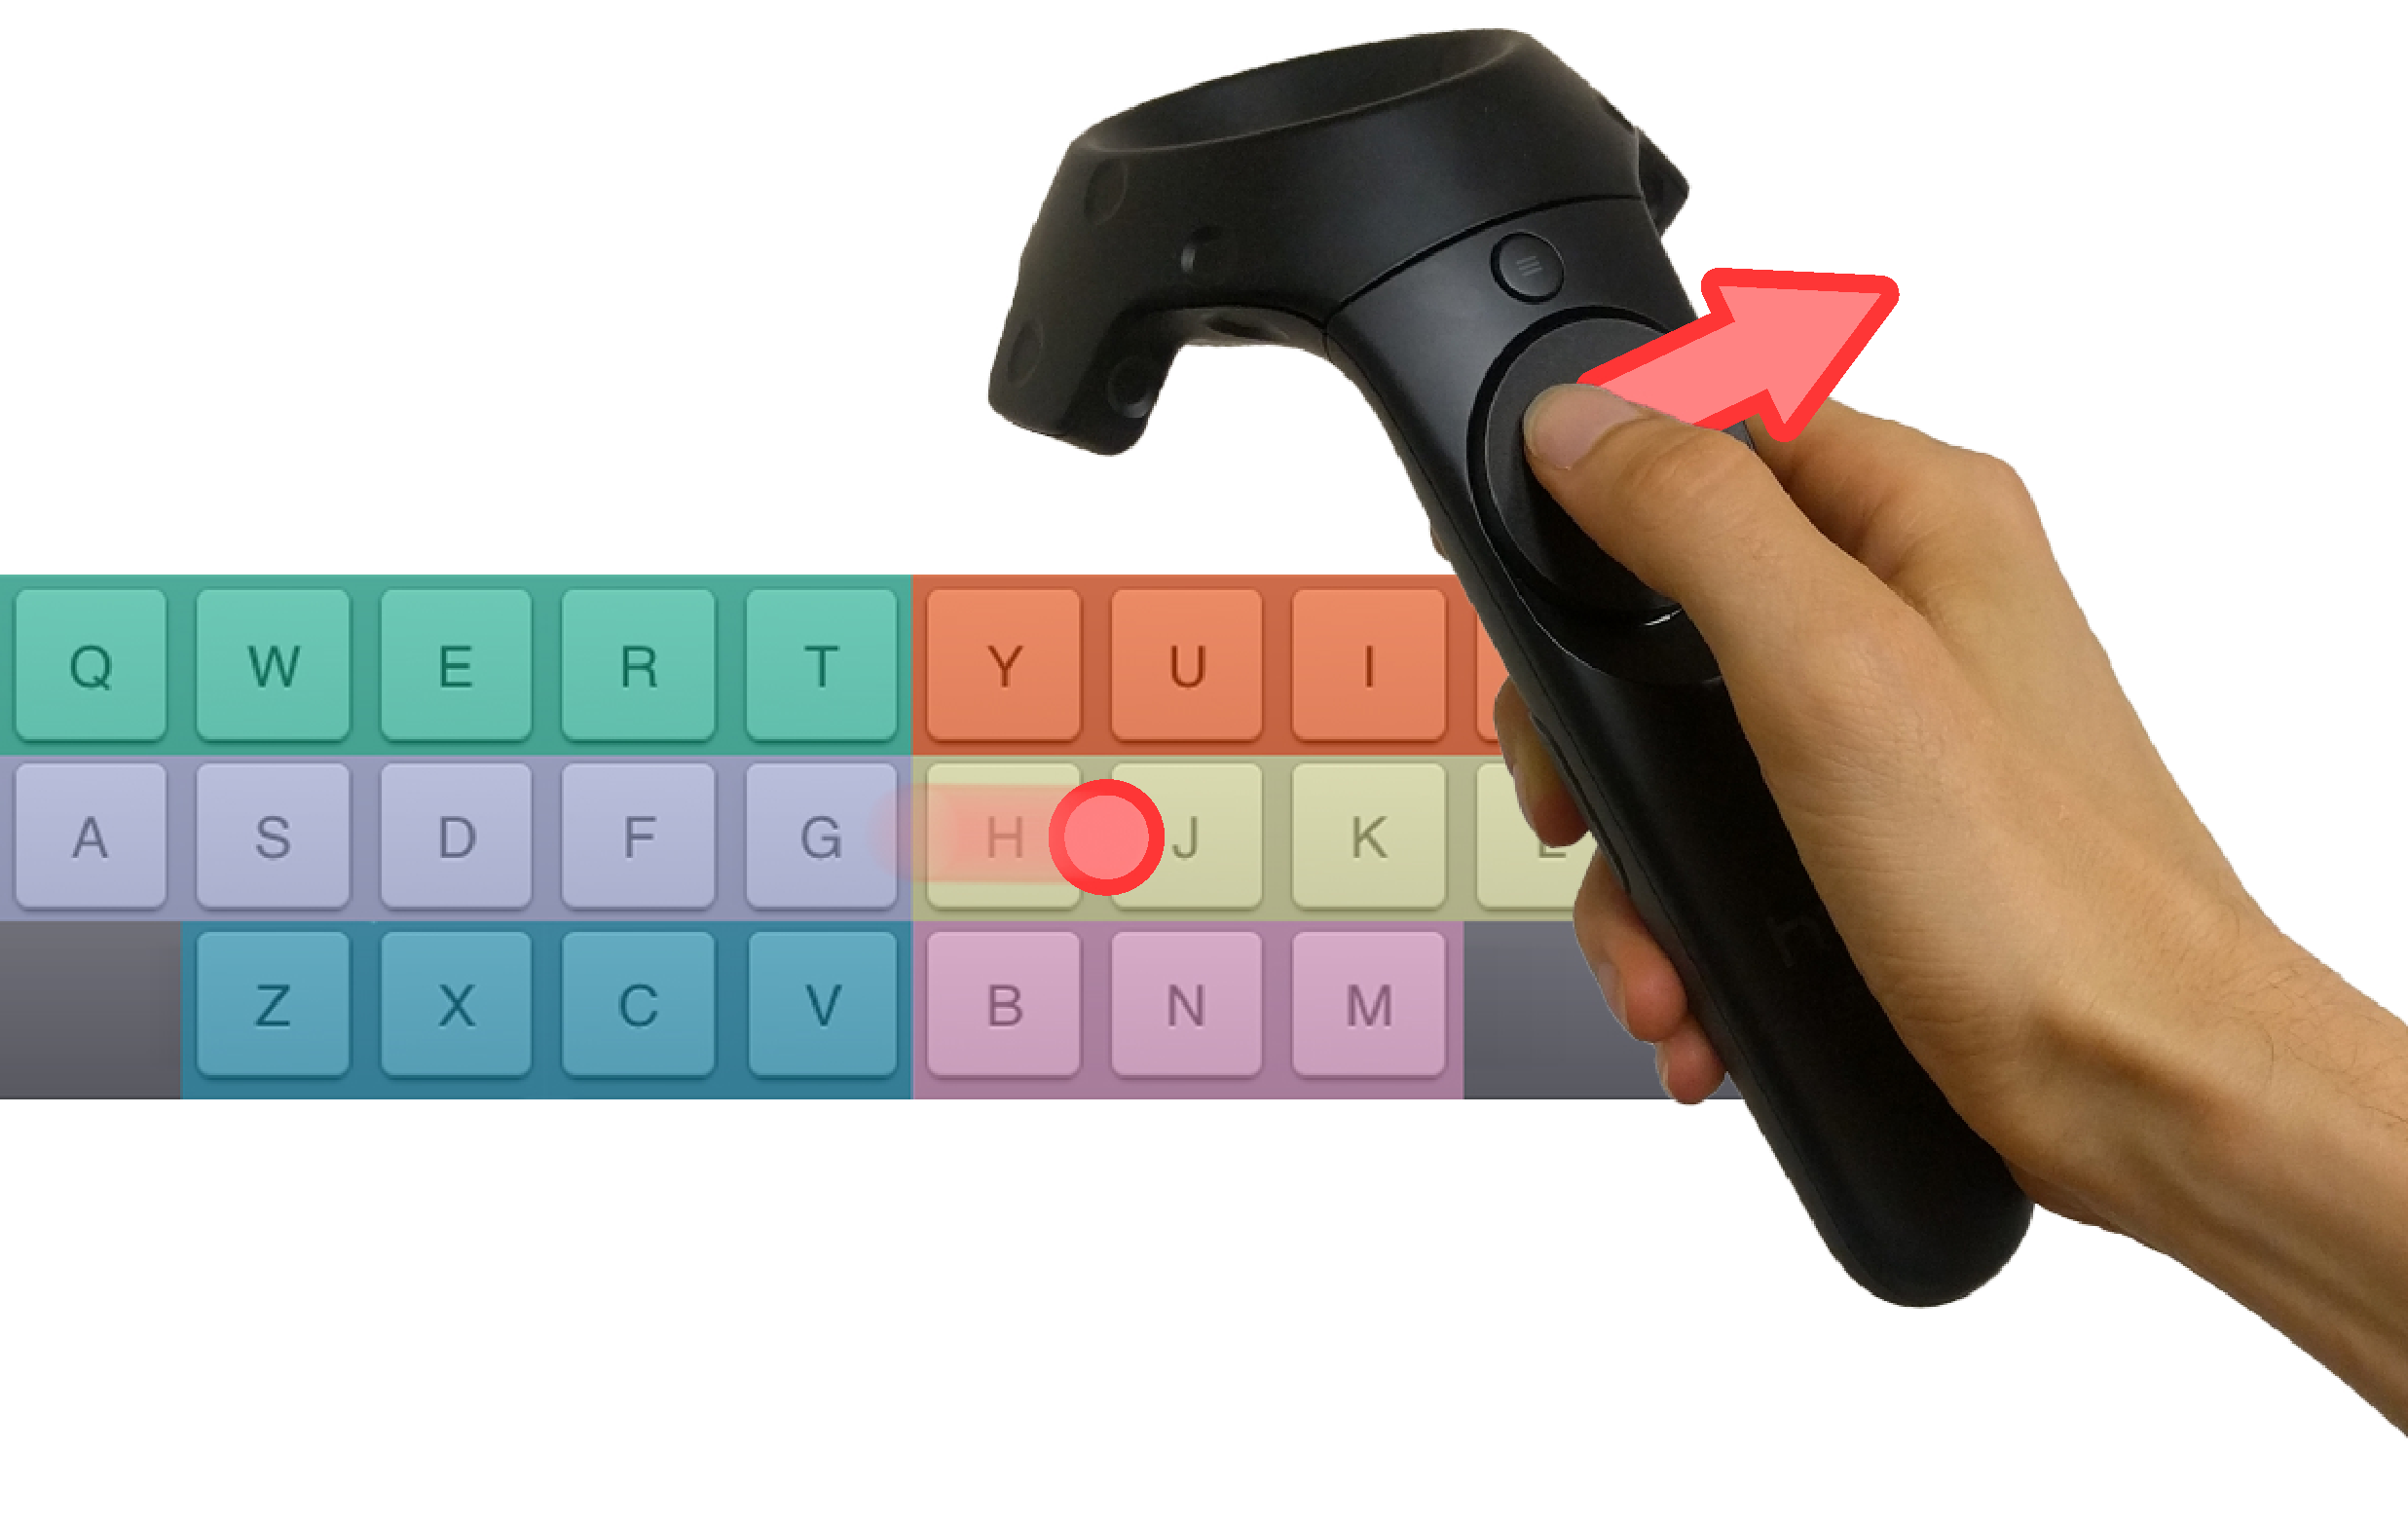
\includegraphics[width=\textwidth]{figures/right}
  \caption{Slide right to enter \textit{l}. }
  \label{fig:controllerVive}
  \end{subfigure}
  \\

  \begin{subfigure}{.6\columnwidth}
  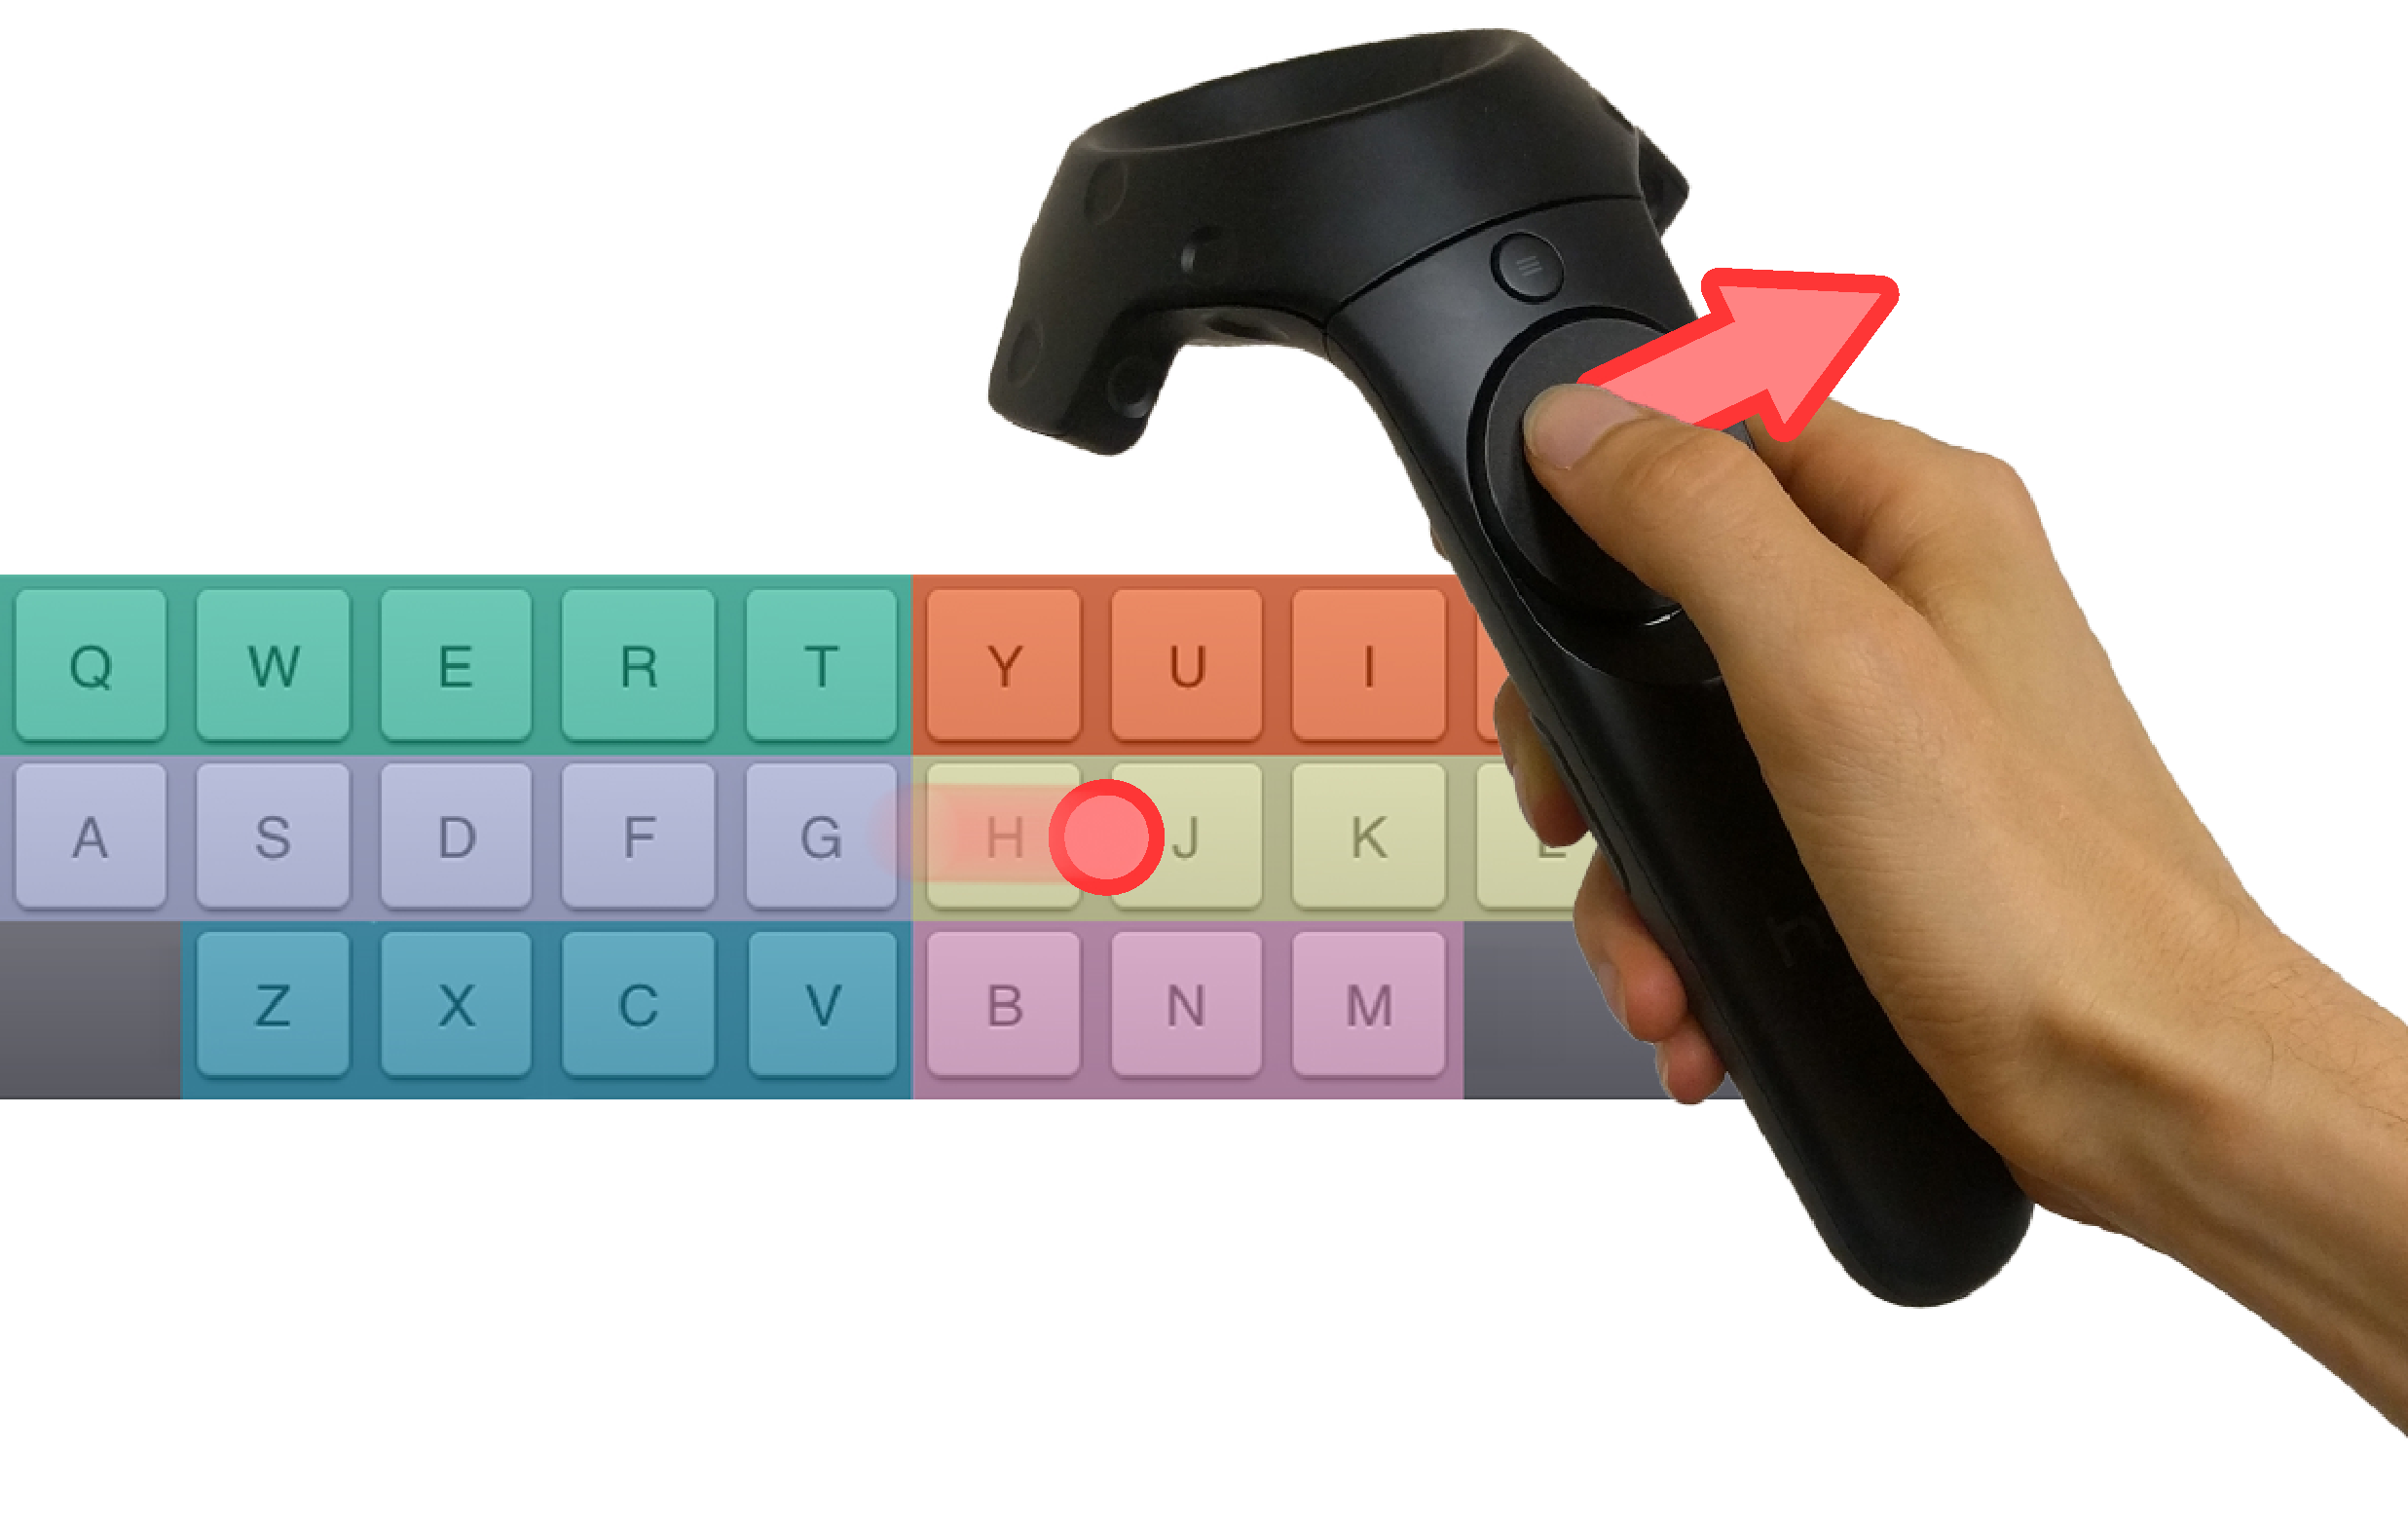
\includegraphics[width=\textwidth]{figures/right}
  \caption{Slide right to enter \textit{l}. }
  \label{fig:controllerVive}
  \end{subfigure}
  \\

  \begin{subfigure}{.6\columnwidth}
  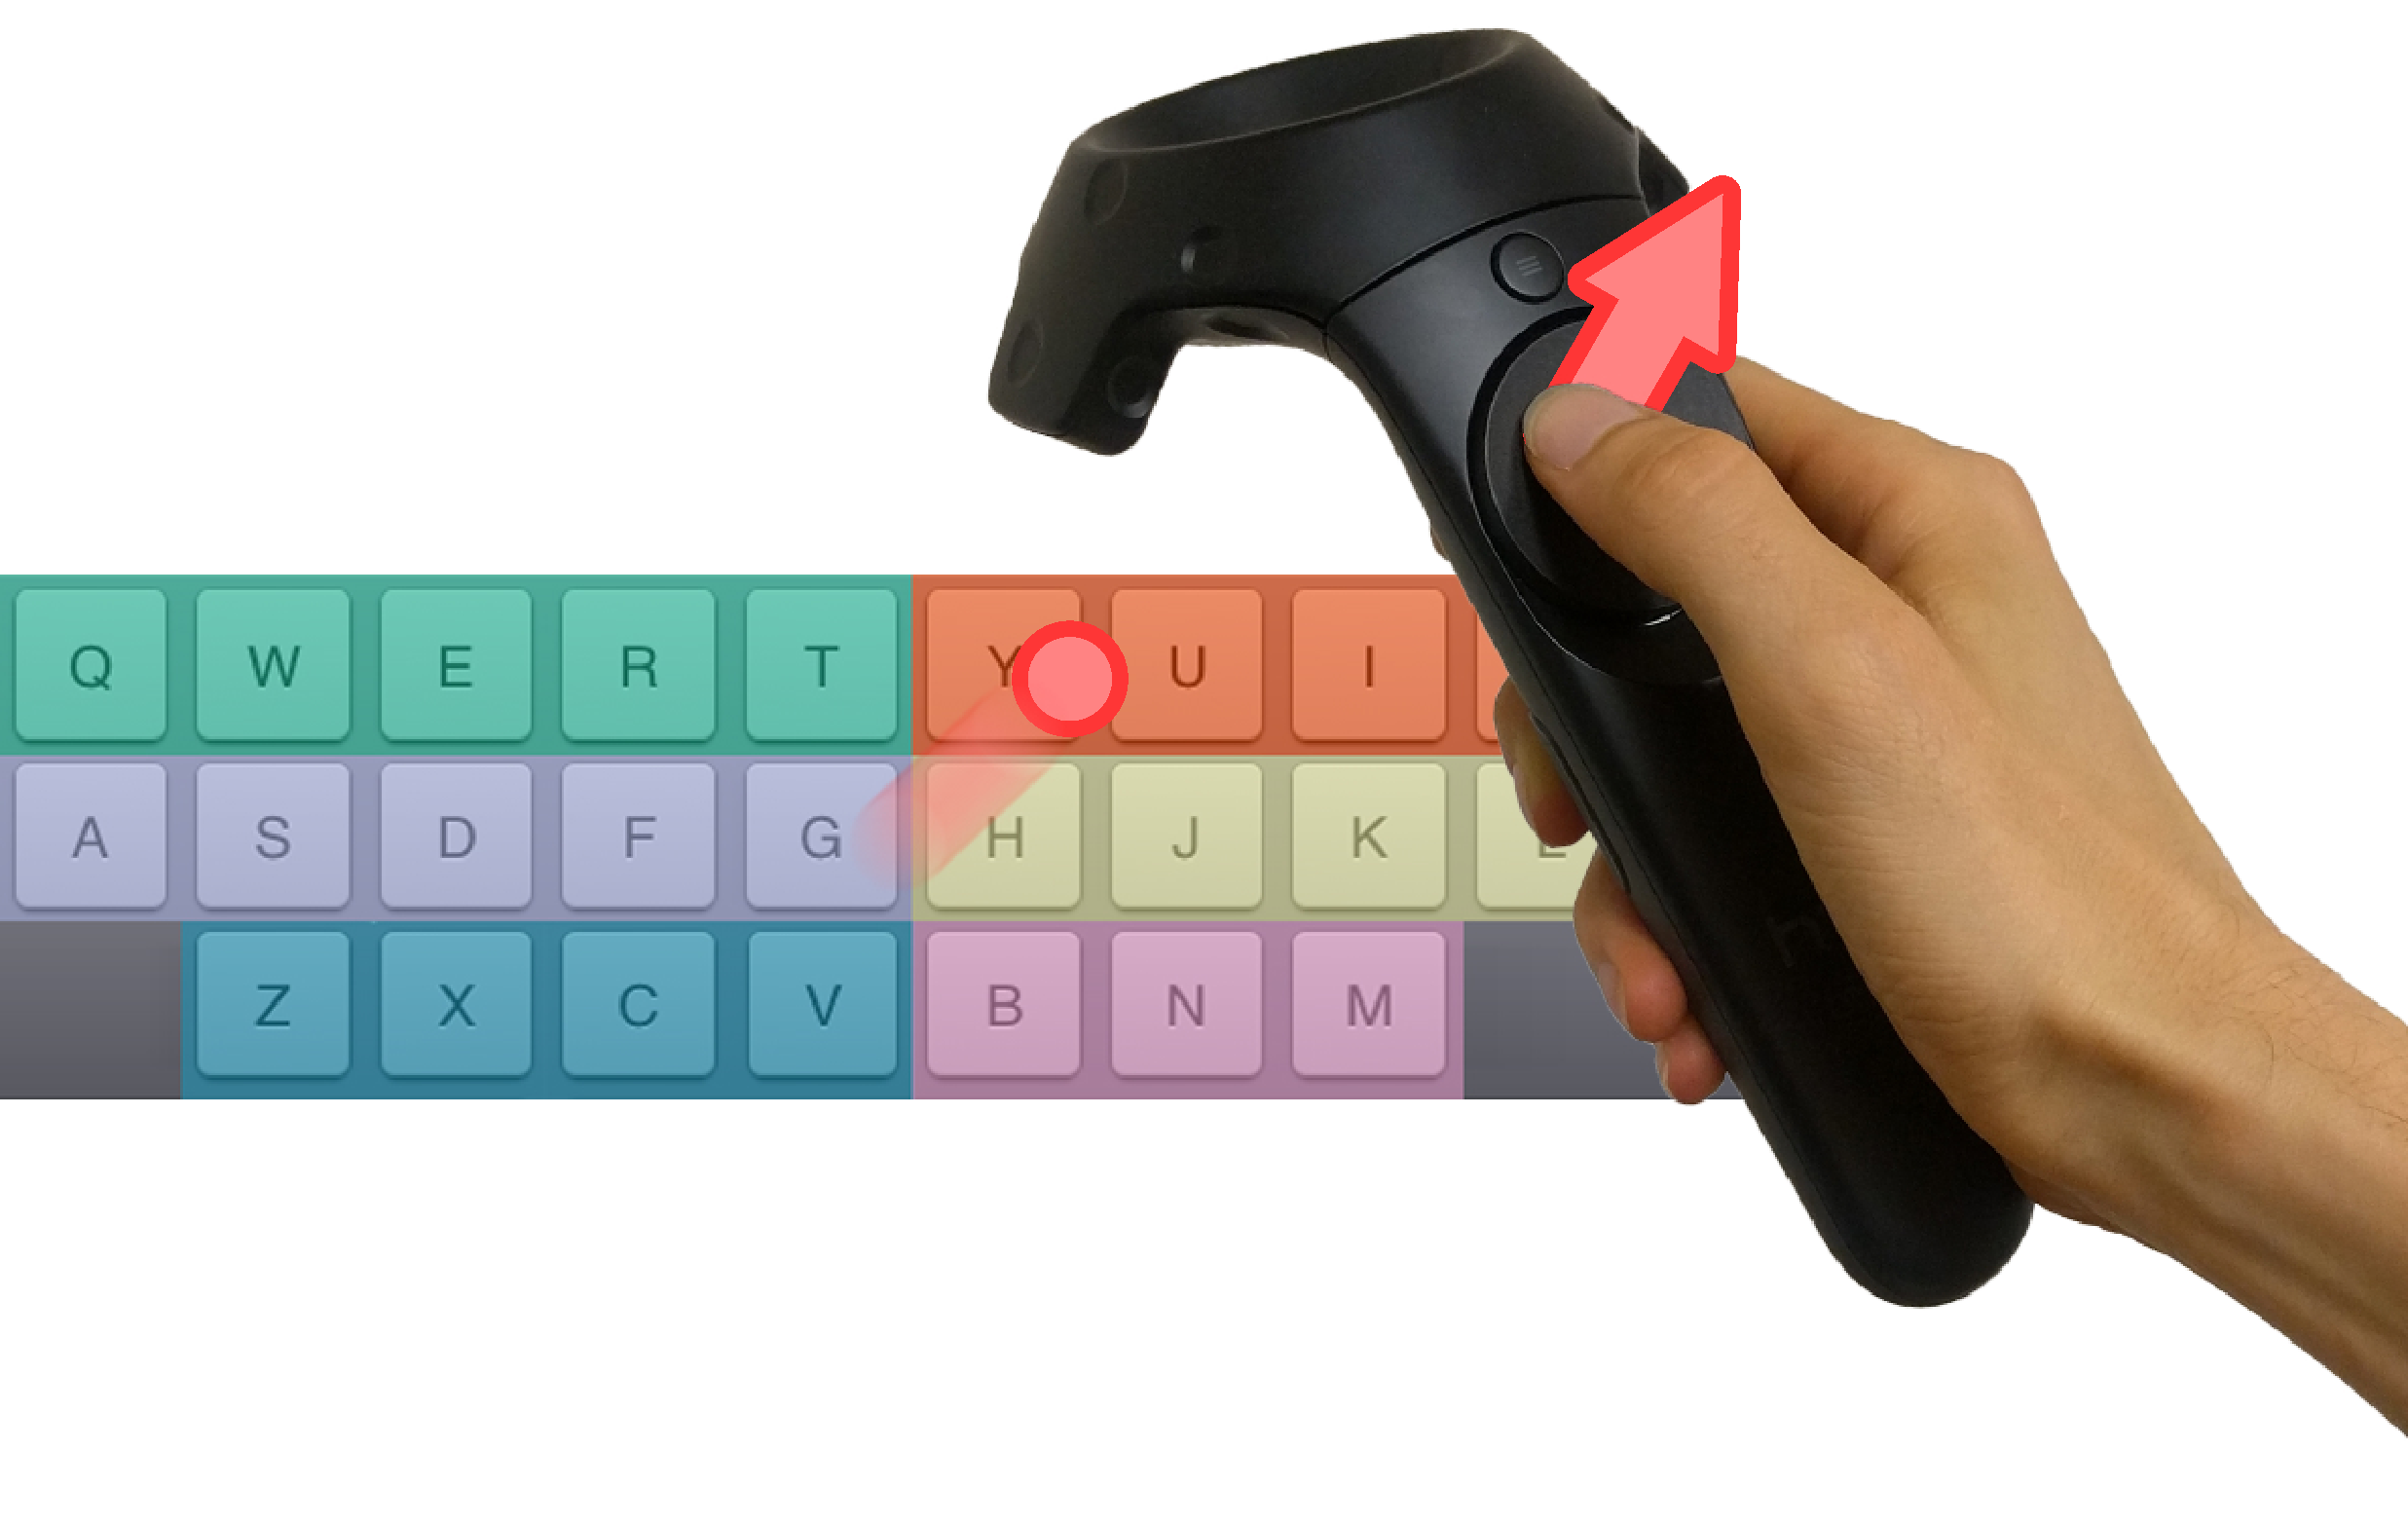
\includegraphics[width=\textwidth]{figures/upperRight}
  \caption{Slide right to enter \textit{o}. }
  \label{fig:controllerVive}
  \end{subfigure}
  \\

  \caption{An example of how the word \textit{hello} is entered using Slide.
  }
~\label{fig:example}

\end{figure}



\begin{comment}

\begin{figure}
\centering

  \begin{tikzpicture}

  \def \n {5}
  \def \radius {3cm}
  \def \margin {8} % margin in angles, depends on the radius

  \foreach \s in {1,...,\n}
  {
    \node[draw, circle] at ({360/\n * (\s - 1)}:\radius) {$\s$};
    \draw[->, >=latex] ({360/\n * (\s - 1)+\margin}:\radius) 
      arc ({360/\n * (\s - 1)+\margin}:{360/\n * (\s)-\margin}:\radius);
    }
  \end{tikzpicture}

  \caption{
    Controller\\
  Intent Detection Classifier\\
    triager \\
  |swipe          |                |\\
    ngram           deterministic     \\
    selection        letter           \\
}~\label{fig:systemFlowchart}
\end{figure}
\end{comment}


\subsection{Variations of Slide}
 
To arrive at the proposed design above, we have tried a few other variations, summarized below. 

\begin{enumerate}
\item
6-tile design and tapping with absolute positioning.  As in Slide, we divide the keys into 6 tiles, and users are asked to just tap on the corresponding tile.  We found that users still cannot hit the right tile, if we adopt absolute positioning.

\item
6-tile design and swiping with absolute positioning.  This design is faster that swiping on a 26-key keyboard, but it is still slower than our proposal. 

\item 
8-tile design with two cursors, and relatively positioning.  Since most people type with two hands on the keyboard, we experimented introducing two cursors into the proposed design.  We split the keyboard into the left and right half, and the initial positions of the left and right thumbs are assumed to be the center of each half.  Instead of sliding to one of 6 directions for each hand, we simplify it to four directions each (up, down, left,  right).  By having 8 rather 6 tiles, this can also reduce the number of ambiguous entries and improve the success of error correction.  

Testing it on a few users quickly pointed out the flaw of this design.  It is too complicated, as the user has to decide which thumb to use, and then which of the four directions.  Furthermore, we found that with the original proposal, the user typically uses the other hand to enter the special the special keys.
\end{enumerate}

Because none of the variations come close to the proposed entry method, our evaluation below focuses primarily on understanding the characteristics of our proposal. 

